\subsubsection{Caso d'uso UC11.1: Inserimento Documentazione API}
\label{UC11.1}
\begin{figure}[ht]
	\centering
	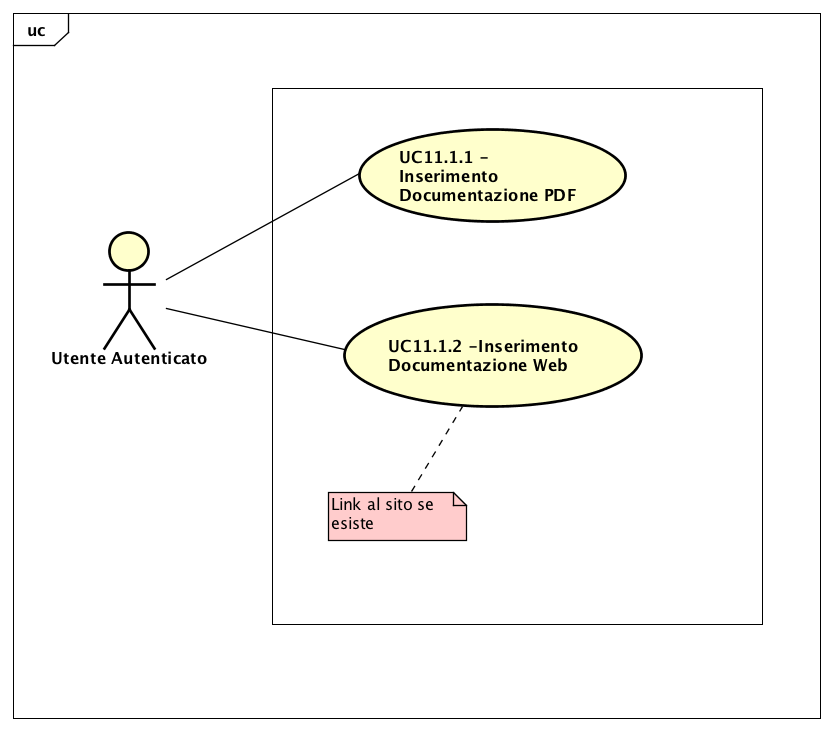
\includegraphics[scale=0.45]{UML/UC11_1.png}
	\caption{Caso d'uso UC11: Registrazione Nuova API}
\end{figure}

\renewcommand*{\arraystretch}{1.6}
\begin{longtable}{ l | p{11cm}}
	\hline
	\rowcolor{Gray}
	\multicolumn{2}{c}{UC11.1: Inserimento Documentazione API} \\
	\hline
	\textbf{Attori} &Utente Autenticato, Amministratore APIMarket \\
	\textbf{Descrizione} & l'attore inserisce la documentazione della propria nuova API \\
	\textbf{Pre-Condizioni} &  l'attore ha scelto di inserire la documentazione della propria nuova API\\
	\textbf{Post-Condizioni}&l'attore ha inserito la documentazione della propria nuova API\\
	\textbf{Scenario Principale} & \begin{enumerate*}[label=(\arabic*.),itemjoin={\newline}]
			\item l'attore può inserire la documentazione della propria nuova API
	\end{enumerate*}\\
\end{longtable}


